
\documentclass[conference]{IEEEtran}

% ---------------------------------------------------------
% PACKAGES
% ---------------------------------------------------------
\usepackage{cite}
\usepackage{amsmath,amssymb,amsfonts}
\usepackage{algorithmic}
\usepackage{algorithm}
\usepackage{array}
\usepackage{booktabs}
\usepackage{multirow}
\usepackage{url}
\usepackage{graphicx}
\usepackage{textcomp}
\usepackage{xcolor}
\usepackage{float}
\usepackage{balance}
\usepackage{tikz}
\usepackage{listings}

\usetikzlibrary{positioning,arrows.meta,shapes.geometric}

% ---------------------------------------------------------
% DOCUMENT
% ---------------------------------------------------------
\begin{document}

% ---------------------------------------------------------
% TITLE
% ---------------------------------------------------------
\title{CropPoint: A Closed-Loop Agricultural Marketplace and
Decision Support System Integrating Multi-Factor Random
Forest Price Forecasting, FAISS-Based RAG, and
Automated Ledger Synchronization}

% ---------------------------------------------------------
% AUTHORS
% ---------------------------------------------------------
\author{
\IEEEauthorblockN{Owesraza Bhati}
\IEEEauthorblockA{
Department of Computer Engineering\\
G H R C E M P\\
Maharashtra, India\\
ansarbhati92@gmail.com}
\and
\IEEEauthorblockN{Nikhil Jaiswar}
\IEEEauthorblockA{
Department of Computer Engineering\\
G H R C E M P\\
Maharashtra, India\\
nikhiljaiswar642@gmail.com}
\and
\IEEEauthorblockN{Mustakim Mansuri}
\IEEEauthorblockA{
Department of Computer Engineering\\
G H R C E M P\\
Maharashtra, India\\
mjmansuri786313@gmail.com}
\and
\IEEEauthorblockN{\hspace*{2.12in}}
\IEEEauthorblockA{}
\and
\IEEEauthorblockN{Mr. Pradeep Taware}
\IEEEauthorblockA{
Department of Computer Engineering\\
G H R C E M P\\
Maharashtra, India\\
pradeep.taware@raisoni.net}
\and
\IEEEauthorblockN{\hspace*{1.5in}}
\IEEEauthorblockA{}
}

\maketitle

% ---------------------------------------------------------
% ABSTRACT
% ---------------------------------------------------------
\begin{abstract}
Smallholder farmers in developing agricultural economies consistently
face income losses caused by intermediary exploitation, information
asymmetry, volatile market prices, and post-harvest logistical
friction. This paper presents CropPoint, also referred to as Smart
Agri AI, a closed-loop agricultural marketplace and decision support
system that connects farmers directly with wholesale and institutional
buyers. The proposed platform combines a machine learning based
price forecasting pipeline, a multi-factor smart price recommendation
mechanism, a Retrieval-Augmented Generation (RAG) advisory subsystem,
and an automated order fulfillment and digital ledger architecture.

The predictive component employs a Random Forest Regressor trained
on 1,351,051 historical Maharashtra Agricultural Produce Market
Committee (APMC) records spanning eight major commodities and
twenty-three years. Twenty-five engineered features representing
temporal behavior, crop seasonality, lagged prices, market arrivals,
rolling statistics, and exponential moving averages are used for
training. The model achieves an $R^2$ score of 0.9687, MAE of
Rs.\,68.40 per quintal, RMSE of Rs.\,94.20, and MAPE of 2.85\%
on a held-out 2024 test set. A hybrid recommendation mechanism then
blends the machine learning output with current mandi prices, EMA
momentum, weekly averages, weather risk, and historical benchmarks.

For agricultural advisory, CropPoint employs Sentence Transformers,
FAISS vector similarity search, and a large language model to
retrieve relevant agricultural knowledge before generating responses.
The advisory system supports English, Hindi, and Marathi. A
four-stage order tracking state machine further connects marketplace
transactions to automated ledger entries upon delivery. The system
therefore integrates price intelligence, agricultural advisory,
direct trade facilitation, logistics tracking, and financial record
management within one unified platform.
\end{abstract}

\begin{IEEEkeywords}
Agricultural marketplace, agricultural price forecasting,
Random Forest, machine learning, retrieval-augmented generation,
FAISS, decision support system, digital ledger, precision
agriculture, e-commerce.
\end{IEEEkeywords}

% =========================================================
% I. INTRODUCTION
% =========================================================
\section{Introduction}

Agriculture contributes substantially to the Indian economy and
sustains the livelihoods of a large rural population. Despite this
importance, agricultural producers regularly encounter difficulties
related to price discovery, market access, dependence on
intermediaries, transportation logistics, weather uncertainty, and
financial record keeping. Small and marginal farmers often have
limited access to reliable real-time market information and
consequently sell produce at prices below prevailing market
levels \cite{chand2012}.

Traditional agricultural supply chains typically involve multiple
intermediaries between the producer and the final buyer. Commission
agents, local traders, and aggregators add transactional complexity
and reduce the farmer's share of the final sale value. Farmers
generally lack simple digital mechanisms for comparing their
expected price with current mandi benchmarks.

Market price volatility compounds these difficulties. Commodity
prices are driven by seasonal production, market arrivals, crop
cycles, regional supply and demand, weather conditions, and
historical price behavior. A single historical average is inadequate
for representing all these interacting factors. Data-driven
forecasting methods, when combined with live market intelligence,
can therefore provide meaningful decision support for agricultural
producers \cite{liakos2018}.

CropPoint is designed to address these interconnected problems
through a unified agricultural information and trading platform.
Rather than treating price forecasting, advisory, marketplace
operations, logistics, and bookkeeping as separate concerns, the
system connects all of them into a single closed-loop workflow.

The principal objectives of CropPoint are:
\begin{enumerate}
    \item To establish a direct farmer-to-buyer agricultural
    marketplace.
    \item To estimate reasonable crop prices using machine learning
    and live market intelligence.
    \item To provide agricultural advisory through a multilingual
    retrieval-augmented generation architecture.
    \item To support purchase requests and structured order
    fulfillment.
    \item To track delivery progression using a four-stage state
    machine.
    \item To automatically synchronize completed sales with the
    farmer's digital ledger.
    \item To surface market and weather information for improved
    agricultural decision making.
\end{enumerate}

The system is implemented using a React-based frontend and a FastAPI
backend. SQLAlchemy is used for asynchronous database operations,
while machine learning functionality is implemented with Scikit-learn
and PyTorch. The RAG subsystem uses Sentence Transformers, FAISS,
and a large language model \cite{lewis2020}.

The primary contribution of this work is not a single prediction
model but the integration of multiple intelligent components into a
closed-loop agricultural workflow. The system progresses from
\emph{market intelligence} to \emph{price recommendation}, from
\emph{buyer request} to \emph{delivery}, and from \emph{delivery}
to \emph{financial record generation}.

The remainder of this paper is organized as follows. Section~II
reviews related work. Section~III describes the system architecture.
Section~IV presents the price forecasting model and hybrid
recommendation engine. Section~V presents the RAG-based advisory
subsystem. Section~VI explains the marketplace, order fulfillment,
and ledger architecture. Section~VII addresses security and database
design. Section~VIII presents the experimental evaluation.
Section~IX discusses limitations and future directions, and
Section~X concludes the paper.

% =========================================================
% II. RELATED WORK
% =========================================================
\section{Related Work}

Agricultural price prediction has attracted research attention from
statistical, machine learning, and deep learning communities.
Classical time-series methods such as ARIMA and exponential smoothing
capture temporal dependencies and seasonality well but may not
adequately model nonlinear relationships between market arrivals,
regional demand, seasonal production cycles, and price levels.

Random Forests provide an ensemble-based approach suited to nonlinear
regression tasks. Breiman introduced the algorithm as a collection
of decision trees trained using bootstrap sampling and random feature
selection \cite{breiman2001}. Their ability to handle mixed
categorical, temporal, and numerical attributes makes them
well-suited to agricultural market datasets. Liakos et al.\
conducted a comprehensive review of machine learning applications
in agriculture and demonstrated the broad applicability of ensemble
methods across crop yield prediction, disease detection, and price
forecasting tasks \cite{liakos2018}.

Deep learning approaches have also been explored for agricultural
time-series forecasting. Long Short-Term Memory (LSTM) networks,
introduced by Hochreiter and Schmidhuber, address the vanishing
gradient problem that limits standard recurrent networks when
learning long-term dependencies \cite{hochreiter1997}. LSTM models
can represent sequential market behavior effectively, though they
require carefully structured temporal inputs and substantial
computational resources during training.

Digital agricultural marketplaces have primarily focused on online
listing, product discovery, and buyer-seller communication. Hisano
et al.\ examined buyer-seller network structures and showed that
market efficiency depends heavily on the connectivity and
transparency of these networks \cite{hisano2017}. Such platforms
improve market accessibility but typically lack integrated
fulfillment tracking, agricultural advisory, and accounting
functionality.

Retrieval-Augmented Generation (RAG) has emerged as an effective
strategy for knowledge-intensive language model applications. Lewis
et al.\ proposed RAG as a framework that combines parametric
language models with external retrieved knowledge to improve
factual accuracy and reduce hallucination \cite{lewis2020}. In an
agricultural context, retrieval can constrain model responses to
relevant crop, pest, market, and government scheme information.

Sentence-BERT provides efficient semantic sentence representations
suitable for similarity search \cite{reimers2019}. FAISS provides
scalable similarity search and clustering over dense vector
representations \cite{johnson2021}.

Ma et al.\ demonstrated that interpretable forecasting systems that
combine statistical models with domain features can achieve strong
predictive performance in agricultural commodity markets
\cite{ma2018}. CropPoint draws on this principle by combining
machine learning prediction with domain-specific market signals.

The present work synthesizes these research directions into a single
application-oriented architecture that integrates machine learning
price prediction, multi-factor recommendation, retrieval-augmented
advisory, direct farmer-buyer trading, delivery state tracking, and
automated digital accounting.

% =========================================================
% III. SYSTEM ARCHITECTURE
% =========================================================
\section{System Architecture}

CropPoint follows a five-layer architecture: presentation, API
gateway, business logic, AI/ML, and persistence. This layering
isolates user interaction, application services, intelligent
processing, and data storage into independently maintainable
components.

\subsection{Presentation Layer}

The presentation layer is implemented using React~18.3 with Vite
and Tailwind~CSS. Role-specific dashboards are provided for
farmers, buyers, and administrators.

The farmer dashboard exposes crop listings, live market information,
AI price recommendations, agricultural advisory, purchase requests,
order tracking, and the digital ledger. The buyer interface provides
marketplace browsing, filtering, buying requirements, purchase
requests, order tracking, invoices, and farmer ratings. The platform
supports English, Hindi, and Marathi through a shared language
context managed at the frontend application level.

\subsection{API Gateway Layer}

The backend is implemented using FastAPI. All versioned REST
endpoints are exposed under the \texttt{/api/v1/} namespace.
Authentication uses JSON Web Tokens (JWT) signed with the HS256
algorithm. Role-based access control differentiates farmers, buyers,
and administrators. Centralized exception handling, request logging,
and input validation are provided through Pydantic-based schemas.

\subsection{Business Logic and AI/ML Layers}

The business logic layer contains domain services for crop listing
management, purchase request handling, deal and order fulfillment,
digital ledger operations, distance and freight calculation,
market-data processing, and scheduled background tasks. The AI/ML
layer contains: Random Forest price regression, PyTorch LSTM
forecasting, EMA trend calculation, hybrid smart price
recommendation, Sentence Transformer embeddings, FAISS vector
search, large language model advisory, multilingual RAG processing,
and weather risk scoring.

\subsection{Persistence Layer}

The persistence layer uses SQLite with SQLAlchemy~2.0 asynchronous
operations. The relational schema contains entities for users, crop
listings, purchase requests, deals, transactions, ledger entries,
farm plots, ratings, notifications, market prices, and weather
cache. External data sources include AGMARKNET APMC market prices
and OpenWeatherMap weather information.

\begin{figure}[htbp]
\centering
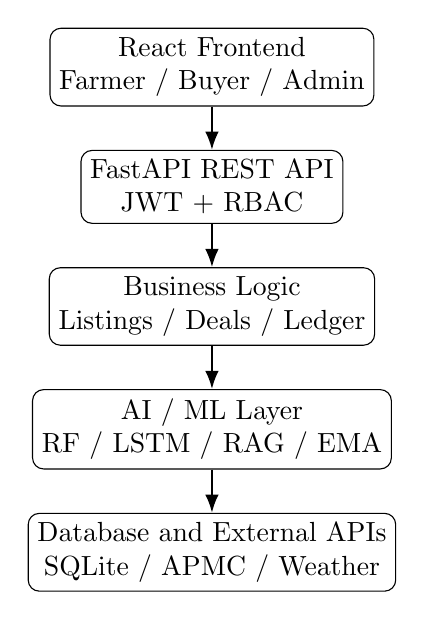
\begin{tikzpicture}[
    node distance=0.55cm,
    box/.style={
        rectangle, draw, rounded corners,
        align=center,
        minimum width=3.0cm,
        minimum height=0.65cm
    },
    arrow/.style={-Latex, thick}
]
\node[box] (frontend) {React Frontend\\Farmer / Buyer / Admin};
\node[box, below=of frontend] (api)   {FastAPI REST API\\JWT + RBAC};
\node[box, below=of api]     (logic)  {Business Logic\\Listings / Deals / Ledger};
\node[box, below=of logic]   (ai)     {AI / ML Layer\\RF / LSTM / RAG / EMA};
\node[box, below=of ai]      (db)     {Database and External APIs\\SQLite / APMC / Weather};
\draw[arrow] (frontend) -- (api);
\draw[arrow] (api)      -- (logic);
\draw[arrow] (logic)    -- (ai);
\draw[arrow] (ai)       -- (db);
\end{tikzpicture}
\caption{Layered architecture of the CropPoint platform.}
\label{fig:architecture}
\end{figure}

% =========================================================
% IV. MULTI-FACTOR AI PRICE RECOMMENDATION
% =========================================================
\section{Multi-Factor AI Price Recommendation}

A central component of CropPoint is the smart price recommendation
engine, which provides a defensible selling price estimate rather
than directly exposing a raw machine learning prediction.

\subsection{Dataset and Temporal Split}

The Random Forest model is trained on 1,351,051 historical
Maharashtra APMC records covering eight major agricultural
commodities: Onion, Wheat, Tomato, Cotton, Soybean, Potato, Rice,
and Maize. The dataset spans 2001 to 2024. A strictly chronological
split is applied to prevent temporal data leakage:
\begin{itemize}
    \item 2001--2021: training set,
    \item 2022--2023: validation set,
    \item 2024: held-out test set.
\end{itemize}
This temporal methodology is essential because allowing future
observations to influence historical training produces unrealistically
optimistic evaluation metrics.

\subsection{Feature Engineering}

Twenty-five features are engineered from the raw agricultural market
data and grouped into four categories.

\textbf{Categorical features:} commodity identifier, district
identifier, market identifier.

\textbf{Calendar and seasonal features:} year, month, day, day of
week, day of year, quarter, Kharif indicator, Rabi indicator, Zaid
indicator.

\textbf{Autoregressive features:} modal price at lag $t{-}1$,
$t{-}3$, $t{-}7$, $t{-}14$, and $t{-}30$.

\textbf{Statistical and momentum features:} logarithmic arrival
volume, price spread, seven-day rolling mean, seven-day rolling
standard deviation, thirty-day rolling mean, EMA-7, EMA-14, EMA-30.

The Exponential Moving Average for window $N$ is computed as:
\begin{equation}
    \mathrm{EMA}_t = \alpha\, P_{t} + (1-\alpha)\,\mathrm{EMA}_{t-1}
\end{equation}
where the smoothing factor is:
\begin{equation}
    \alpha = \frac{2}{N+1}
\end{equation}

\subsection{Random Forest Model}

The primary regression model is a Random Forest Regressor containing
100 decision trees with the following hyperparameters:
\texttt{n\_estimators}~=~100, \texttt{max\_depth}~=~20,
\texttt{min\_samples\_split}~=~5, \texttt{min\_samples\_leaf}~=~2,
\texttt{random\_state}~=~42, and \texttt{n\_jobs}~=~$-1$.

The ensemble prediction is the average of individual tree predictions:
\begin{equation}
    \hat{y} = \frac{1}{T}\sum_{t=1}^{T} f_t(\mathbf{X})
\end{equation}
where $T$ is the number of trees and $f_t(\mathbf{X})$ is the
prediction of the $t$-th tree on feature vector $\mathbf{X}$.

\subsection{Benchmark Results}

The Random Forest model is evaluated against a Linear Regression
baseline and a two-layer PyTorch LSTM model.

\begin{table}[htbp]
\centering
\caption{Regression Model Performance on 2024 Test Set}
\label{tab:results}
\begin{tabular}{lcccc}
\toprule
\textbf{Model} & $R^2$ & MAE & RMSE & MAPE \\
\midrule
Linear Regression      & 0.8124 & 184.20 & 248.50 & 8.45\% \\
PyTorch LSTM           & 0.9412 &  89.60 & 118.40 & 3.65\% \\
\textbf{Random Forest} & \textbf{0.9687} & \textbf{68.40} &
\textbf{94.20} & \textbf{2.85\%} \\
\bottomrule
\end{tabular}
\end{table}

The Random Forest achieves the strongest performance, with an $R^2$
of 0.9687 indicating that the model accounts for a high proportion
of price variance on the held-out test data. The MAPE of 2.85\%
represents the lowest relative error among all evaluated models.

\subsection{Hybrid Smart Price Formula}

The system does not expose the raw machine learning prediction.
Instead, six market signals are blended using a weighted formula:
\begin{equation}
\begin{aligned}
P_{\mathrm{rec}} ={}&
  0.35\,P_{\mathrm{mandi}}
+ 0.25\,P_{\mathrm{ML}}
+ 0.20\,P_{\mathrm{EMA}}\\
&+ 0.10\,P_{\mathrm{week}}
+ 0.05\,P_{\mathrm{weather}}
+ 0.05\,P_{\mathrm{hist}}
\end{aligned}
\label{eq:hybrid}
\end{equation}
where $P_{\mathrm{mandi}}$ is the current modal mandi price,
$P_{\mathrm{ML}}$ is the Random Forest prediction,
$P_{\mathrm{EMA}}$ is the momentum-adjusted EMA price,
$P_{\mathrm{week}}$ is the seven-day average,
$P_{\mathrm{weather}}$ is the weather-adjusted price, and
$P_{\mathrm{hist}}$ is the historical monthly baseline.

The EMA component is adjusted according to market direction: an
upward trend applies a multiplier of 1.02, while a downward trend
applies 0.98. A rain probability exceeding 60\% reduces the weather
factor to 0.97; low-risk conditions allow a factor of 1.02. A
quality multiplier $Q$ produces the final price:
\begin{equation}
    P_{\mathrm{final}} = P_{\mathrm{rec}} \times Q
\end{equation}
where Grade A corresponds to $Q = 1.02$ and Grade C to $Q = 0.95$.

% =========================================================
% V. RETRIEVAL-AUGMENTED AGRICULTURAL ADVISORY
% =========================================================
\section{Retrieval-Augmented Agricultural Advisory}

Numerical price regression is unsuitable for open-ended agricultural
questions. Farmers may enquire about crop diseases, pest management,
cultivation practices, government schemes, or market strategy.
CropPoint therefore implements a Retrieval-Augmented Generation
architecture for agricultural advisory.

\subsection{Knowledge Base and Embedding}

The agricultural knowledge base consists of 17 curated documents
covering eight major crops, including crop calendars, pest and
disease information, market guidance, and government scheme
summaries. An incoming query is encoded into a dense vector using
the Sentence Transformers \texttt{all-MiniLM-L6-v2} model, producing
a 384-dimensional embedding:
\begin{equation}
    d = 384
\end{equation}

\subsection{FAISS Similarity Search}

The query embedding is matched against the document index using a
FAISS \texttt{IndexFlatIP} structure. Because all vectors are
L2-normalized, inner-product similarity is equivalent to cosine
similarity. For vectors $\mathbf{x}$ and $\mathbf{y}$:
\begin{equation}
    \cos(\mathbf{x},\mathbf{y}) =
    \frac{\mathbf{x}\cdot\mathbf{y}}{\|\mathbf{x}\|\,\|\mathbf{y}\|}
\end{equation}
After normalization this simplifies to:
\begin{equation}
    \cos(\mathbf{x},\mathbf{y}) = \mathbf{x}\cdot\mathbf{y}
\end{equation}
The system retrieves the top-3 most similar knowledge chunks. A
cosine similarity threshold of 0.45 is applied; queries falling
below this threshold receive a structured fallback response
directing the farmer to the nearest Krishi Vigyan Kendra.

\subsection{Context Injection and Language Model Generation}

Retrieved document chunks are concatenated and injected as context
into the language model prompt:
\begin{verbatim}
Context: {retrieved_chunks}
Query:   {user_query}
\end{verbatim}
The complete RAG pipeline can be expressed as:
\begin{equation}
\mathrm{Query}
\xrightarrow{\text{embed}}
\mathrm{FAISS}
\xrightarrow{\text{top-3}}
\mathrm{Context}
\xrightarrow{\text{LLM}}
\mathrm{Response}
\end{equation}
This approach grounds responses in the curated agricultural knowledge
base rather than relying on unconstrained open-domain generation.

\subsection{Multilingual Support}

The advisory system supports English, Hindi, and Marathi. Backend
prompt templates instruct the language model to generate responses
in the selected language, with Hindi and Marathi responses produced
in Devanagari script. This multilingual design is essential for
Indian agricultural applications where farmers are often more
comfortable in their native language \cite{chand2012}.

% =========================================================
% VI. MARKETPLACE, ORDER FULFILLMENT, AND LEDGER
% =========================================================
\section{Marketplace, Order Fulfillment, and Ledger}

\subsection{Direct Agricultural Marketplace}

CropPoint provides a B2B marketplace connecting farmers with
wholesale and institutional buyers. A farmer creates a crop listing
specifying crop name, quantity in quintals, expected price, quality
grade, location, and optional advance booking period. Listings are
stored in the \texttt{crop\_listings} table, with ownership checks
applied before any mutation operation.

Buyers browse active listings, apply crop and quality filters, and
submit purchase requests. An AI-assisted negotiation mechanism
allows the smart-price endpoint to be invoked in buyer mode to
estimate a reasonable counter-bid based on live market conditions.

When a farmer accepts a purchase request, the system creates a
corresponding deal record that serves as the central object for
fulfillment tracking, invoicing, and ledger synchronization:
\begin{equation}
\mathrm{Listing}
\rightarrow \mathrm{PurchaseRequest}
\rightarrow \mathrm{Accepted}
\rightarrow \mathrm{Deal}
\end{equation}

\subsection{Four-Stage Order Fulfillment State Machine}

The active order workflow follows four sequential states:
(1)~Order Confirmed, (2)~Dispatched, (3)~Out for Delivery,
(4)~Delivered. The first transition occurs when the farmer accepts
the buyer's purchase request. The second and third transitions are
initiated by the farmer as physical dispatch and transit progress.
The fourth transition records successful delivery.

\begin{figure}[htbp]
\centering
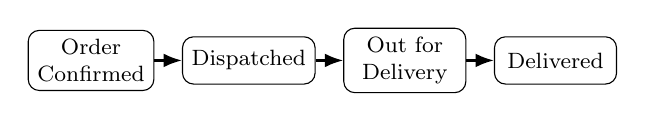
\begin{tikzpicture}[
    node distance=0.35cm,
    state/.style={
        rectangle, draw, rounded corners,
        align=center,
        minimum width=1.55cm,
        minimum height=0.6cm,
        font=\footnotesize
    },
    arrow/.style={-Latex, thick}
]
\node[state] (s1) {Order\\Confirmed};
\node[state, right=of s1] (s2) {Dispatched};
\node[state, right=of s2] (s3) {Out for\\Delivery};
\node[state, right=of s3] (s4) {Delivered};
\draw[arrow] (s1) -- (s2);
\draw[arrow] (s2) -- (s3);
\draw[arrow] (s3) -- (s4);
\end{tikzpicture}
\caption{Four-stage CropPoint order fulfillment state machine.}
\label{fig:state}
\end{figure}

Each transition is timestamped and triggers a buyer notification.
Distance between farm and delivery location is estimated using the
Haversine formula:
\begin{equation}
d = 2R\arcsin\!\left(\sqrt{
    \sin^2\!\left(\tfrac{\Delta\phi}{2}\right)
    + \cos\phi_1\cos\phi_2\sin^2\!\left(\tfrac{\Delta\lambda}{2}\right)
}\right)
\label{eq:haversine}
\end{equation}
where $R = 6{,}371$\,km. A road correction factor of 1.25 is
applied to convert great-circle distance to approximate road
distance:
\begin{equation}
    d_{\mathrm{road}} = 1.25\,d
\end{equation}

Delivery estimates follow distance slabs as shown in
Table~\ref{tab:distance}. The current implementation does not
incorporate real-time GPS routing or traffic information.

\begin{table}[htbp]
\centering
\caption{Distance-Based Delivery Estimation}
\label{tab:distance}
\begin{tabular}{cc}
\toprule
\textbf{Distance (km)} & \textbf{Estimated Delivery} \\
\midrule
0--100     & 1 day  \\
101--300   & 2 days \\
301--500   & 3 days \\
501--800   & 4 days \\
$>$800     & 5 days \\
\bottomrule
\end{tabular}
\end{table}

Freight cost is estimated as:
\begin{equation}
    C_f = d_{\mathrm{road}} \times 0.50 \times Q_{\mathrm{qtl}}
\end{equation}
where $Q_{\mathrm{qtl}}$ is the shipment quantity in quintals.

\subsection{Automated Digital Ledger Synchronization}

When a deal reaches the \texttt{Delivered} state, the system
automatically generates a transaction record, a downloadable invoice,
and a corresponding ledger entry categorized as
\emph{Crop Sale (Marketplace)}:
\begin{equation}
\mathrm{Delivered}
\rightarrow \mathrm{Transaction}
\rightarrow \mathrm{Invoice}
\rightarrow \mathrm{Ledger}
\end{equation}
Net profit is recorded as:
\begin{equation}
    \mathrm{NetProfit} = \mathrm{TotalSaleAmount} - \mathrm{TransportCost}
\end{equation}
This automation removes the need for the farmer to manually record
completed marketplace sales, creating a verifiable chain from trade
confirmation to financial record.

% =========================================================
% VII. SECURITY AND DATABASE DESIGN
% =========================================================
\section{Security and Database Design}

\subsection{Authentication and Access Control}

The platform uses JWT bearer authentication with HS256 signing.
Passwords are stored using BCrypt with a cost factor of 12.
Three primary roles are implemented: Farmer, Buyer, and
Administrator. Farmers can create listings, advance deal stages,
and access their own ledger. Buyers can browse listings and submit
purchase requests. Administrators have platform-level monitoring
access.

Ownership checks are applied to all mutation endpoints, preventing
Insecure Direct Object Reference (IDOR) attacks. Unauthorized
access returns an HTTP~403 response. Database access is performed
exclusively through SQLAlchemy ORM expressions rather than raw
string concatenation, mitigating SQL injection risk.

\subsection{Relational Database Schema}

The persistence layer contains 22 relational tables. The primary
chain of relationships is:
\begin{equation}
\begin{split}
\mathrm{User}
\rightarrow \mathrm{Listing}
&\rightarrow \mathrm{PurchaseRequest}
\rightarrow \mathrm{Deal}\\
&\rightarrow \mathrm{Transaction}
\rightarrow \mathrm{Ledger}
\end{split}
\end{equation}
Additional entities include \texttt{buyer\_profiles},
\texttt{offers}, \texttt{plots}, \texttt{ratings},
\texttt{notifications}, \texttt{market\_prices},
\texttt{weather\_cache}, \texttt{analytics}, and
\texttt{refresh\_tokens}. Cascading foreign key constraints
maintain referential integrity across all tables.

% =========================================================
% VIII. EXPERIMENTAL EVALUATION
% =========================================================
\section{Experimental Evaluation}

\subsection{Functional Test Suite}

A comprehensive test suite of 68 test cases was executed against
the live system across 13 functional modules. The suite covers:
API health verification, invalid token rejection, role-based access
enforcement, farmer listing creation, IDOR attack prevention,
buyer purchase request creation, deal creation, delivery state
transitions, automatic ledger synchronization, duplicate rating
prevention, smart-price recommendation verification, regional
demand retrieval, and RAG-based agricultural question answering.

\begin{table}[htbp]
\centering
\caption{Module-Level Functional Test Results}
\label{tab:tests}
\begin{tabular}{lcc}
\toprule
\textbf{Module} & \textbf{Tests} & \textbf{Passed} \\
\midrule
Health \& Root            &  4 &  4 \\
Authentication (JWT)      &  7 &  7 \\
Farm Plot Management      &  4 &  4 \\
Market / AGMARKNET        &  8 &  8 \\
Weather (OpenWeatherMap)  &  3 &  3 \\
Crop Listings             &  4 &  4 \\
AI Engine (RAG + ML)      &  8 &  8 \\
Deals Lifecycle           &  2 &  2 \\
Ledger \& Workflow        &  7 &  7 \\
Analytics \& Dashboard    &  6 &  6 \\
Notifications \& Reports  &  4 &  4 \\
Marketplace \& Offers     & 10 &  9 \\
Frontend Build            &  1 &  1 \\
\midrule
\textbf{Total}            & \textbf{68} & \textbf{67} \\
\bottomrule
\end{tabular}
\end{table}

The overall pass rate is 98.5\% across 68 functional tests. The
single failure corresponds to a route canonicalization issue
(\texttt{/requirements} without trailing slash returns HTTP~405;
\texttt{/requirements/} returns HTTP~200), which does not affect
frontend operation since the frontend uses the correct canonical
path.

\subsection{Machine Learning Evaluation}

As shown in Table~\ref{tab:results}, the Random Forest model achieves
an $R^2$ of 0.9687 and a MAPE of 2.85\%, outperforming both the
linear regression baseline and the evaluated LSTM model on the
chronological 2024 test set. The combination of categorical,
calendar, autoregressive, rolling, arrival, and momentum features
provides substantial predictive signal for the historical market
dataset.

These results should be interpreted as evaluation metrics for the
specified dataset and temporal configuration rather than guaranteed
forecasts of future agricultural commodity prices.

% =========================================================
% IX. LIMITATIONS AND FUTURE WORK
% =========================================================
\section{Limitations and Future Work}

\subsection{Current Limitations}

Several limitations of the current implementation must be
acknowledged. First, delivery distance is approximated using the
Haversine formula between district centroids with a fixed road
factor; real-time GPS routing, tolls, and traffic conditions are
not incorporated. Second, the frontend uses HTTP polling rather
than persistent WebSocket connections, which can produce unnecessary
network traffic when no state changes have occurred. Third, live
mandi information depends on external API availability, with a
local historical dataset serving as fallback. Fourth, financial
settlement is represented through transaction and ledger records;
live payment escrow and bank integration are not implemented.
Fifth, the deployment uses SQLite, suitable for single-node
environments but requiring migration to a distributed database for
high-concurrency production use. Finally, the RAG knowledge base
is limited to its 17 curated documents; out-of-domain queries may
not receive adequately grounded responses.

\subsection{Future Directions}

Future work can extend CropPoint along several dimensions.
Smart contract-based escrow using blockchain technology can hold
buyer funds and release payment after verified delivery, with IoT
sensors providing tamper-evident delivery evidence. A computer
vision subsystem can identify crop diseases and pests from uploaded
leaf images, with the diagnosis injected into the RAG context to
combine visual and textual agricultural information. Satellite
remote sensing using vegetation indices such as NDVI from Sentinel-2
data can enable plot-level monitoring and improve yield forecasting.
Real-time routing APIs can replace the centroid-based distance
approximation. Finally, feedback collected from farmers after
recommendations and transactions can be used to fine-tune
recommendation strategies through reinforcement learning.

% =========================================================
% X. CONCLUSION
% =========================================================
\section{Conclusion}

This paper presented CropPoint, a closed-loop agricultural
marketplace and decision support platform designed to address
intermediary dependence, price uncertainty, information asymmetry,
fulfillment friction, and manual financial record keeping in
smallholder farming contexts.

The platform integrates a Random Forest agricultural price model
trained on 1,351,051 Maharashtra APMC records with 25 engineered
features. Chronological evaluation on a held-out 2024 test set
shows that the Random Forest achieves an $R^2$ of 0.9687 and a
MAPE of 2.85\%, outperforming the evaluated linear regression and
LSTM baselines. The raw machine learning prediction is not directly
exposed; instead, the six-factor hybrid formula~(\ref{eq:hybrid})
blends the ML output with live mandi prices, EMA momentum, weekly
averages, weather risk, and historical benchmarks.

For agricultural advisory, the RAG architecture uses Sentence
Transformer embeddings and FAISS similarity search to retrieve
relevant knowledge before generating multilingual responses in
English, Hindi, and Marathi. The direct farmer-buyer marketplace
and four-stage order fulfillment workflow connect market intelligence
to physical trade. Crucially, reaching the Delivered state
automatically triggers transaction record creation and ledger
synchronization, establishing a verifiable chain from trade to
financial record:
\begin{equation}
\mathrm{Trade}
\rightarrow \mathrm{Fulfillment}
\rightarrow \mathrm{Delivery}
\rightarrow \mathrm{FinancialRecord}
\end{equation}

Functional testing across 68 test cases yielded a 98.5\% pass rate.
Future development can extend the platform with smart-contract
escrow, computer vision, satellite monitoring, real-time logistics,
and reinforcement learning from farmer feedback.

Overall, CropPoint demonstrates that machine learning,
retrieval-augmented generation, agricultural market intelligence,
e-commerce, logistics tracking, and digital accounting can operate
as interconnected components of a single agricultural
decision-support ecosystem, producing measurable value for
smallholder farmers who currently lack access to integrated
digital tools.

% =========================================================
% REFERENCES
% =========================================================
\begin{thebibliography}{00}

\bibitem{chand2012}
S. Chand,
``Marketing of agricultural produce in India: Role of intermediaries
and price realization for farmers,''
\emph{Indian Journal of Agricultural Economics},
vol.~67, no.~3, 2012.

\bibitem{breiman2001}
L. Breiman,
``Random forests,''
\emph{Machine Learning},
vol.~45, no.~1, pp.~5--32, 2001.

\bibitem{hochreiter1997}
S. Hochreiter and J. Schmidhuber,
``Long short-term memory,''
\emph{Neural Computation},
vol.~9, no.~8, pp.~1735--1780, 1997.

\bibitem{lewis2020}
P. Lewis, E. Perez, A. Piktus, F. Petroni,
V. Karpukhin, N. Goyal, H. K\"{u}ttler,
M. Lewis, W.\nobreakdash-t. Yih, T. Rockt\"{a}schel,
S. Riedel, and D. Kiela,
``Retrieval-augmented generation for knowledge-intensive NLP tasks,''
in \emph{Advances in Neural Information Processing Systems (NeurIPS)},
vol.~33, 2020, pp.~9459--9474.

\bibitem{johnson2021}
J. Johnson, M. Douze, and H. J\'{e}gou,
``Billion-scale similarity search with GPUs,''
\emph{IEEE Transactions on Big Data},
vol.~7, no.~3, pp.~535--547, 2021.

\bibitem{reimers2019}
N. Reimers and I. Gurevych,
``Sentence-BERT: Sentence embeddings using Siamese BERT-networks,''
in \emph{Proc. EMNLP-IJCNLP},
Hong Kong, China, 2019, pp.~3982--3992.

\bibitem{liakos2018}
K. G. Liakos, P. Busato, D. Moshou, S. Pearson, and D. Bochtis,
``Machine learning in agriculture: A review,''
\emph{Sensors},
vol.~18, no.~8, p.~2674, 2018.

\bibitem{hisano2017}
R. Hisano, T. Ohnishi, and T. Watanabe,
``Dynamics of buyer-seller networks in agricultural markets,''
\emph{Applied Network Science},
vol.~2, no.~1, p.~8, 2017.

\bibitem{ma2018}
J. Ma, Z. Liu, Y. Li, and Q. Sun,
``An interpretable produce price forecasting system,''
\emph{Complexity},
vol.~2018, pp.~1--14, 2018.

\bibitem{agmarknet}
Government of India, Ministry of Agriculture and Farmers Welfare,
``Agricultural Marketing Information Network (Agmarknet),''
\url{https://agmarknet.gov.in},
[Online; accessed Sep.\ 2026].

\end{thebibliography}

\balance

\end{document}
